% failuredetection.tex
\documentclass[dareport.tex]{subfiles}
\begin{document}
% Content here
\section{Failure Detection}
Strike system is designed to run with multi-server environment. One of the key challenge for such server cluster is how reliably and efficiently to determine the crashed failure state of the next server member(s). This section discuss how Strike server implement distributed algorithm for reliable failure detection.

\subsection{Naive Approach}

Initially, the Naive approach is used to implement failure detection in Strike Server. Let us assume there are 4 servers cluster in the following discussion for simplicity. Each server will try to establish a short TCP connection to all peer severs at every interval X for checking heartbeat signal. Each server maintains a data structure of \textbf{AliveMap}\footnote{ConcurrentHashMap in Java, with key (String) for server ID and value (Integer) for error count} to store error count for all known servers. i.e. \verb|{"1":0, "2":3, "3":1, "4":2}|. When \verb|server1| fails to establish short TCP connection with \verb|server2|, \verb|server1| will modify its local \textbf{AliveMap} to increase the error count of \verb|server2| by plus 1. When the error count of a particular server reaches to error factor Y, that server is considered as crashed --- (Parameter X and Y can be set in configuration file). A server who detected a failed server will broadcast a message to all other servers to inform them removing the failed server from their \textbf{ServerState} registry. This can be a problem in a partially connected network; a detected "failed server" will be removed from the server list from all other servers since no consensus on removing failure server is met. The consensus improvements will be discussed in consensus section.

Failure detection using Naive approach may works fine in a group of a few servers, however it is not effective when server farm scale to a large number. For $N$ servers, there will be $O(N^{2})$ TCP connections among the servers for every heartbeat interval. This will lead to message explosion\cite{failuredetector}. A good failure detector in large scale distributed system must prevent flooding or overloading the network with failure detection related messages whereas the Naive approach of heartbeat failure detector does not. In this case, a better approach is needed.

\subsection{Gossip Algorithm}

To address this problem, we used gossip-type protocol to implement distributed algorithm in the chat system. In the article "Failure Detectors for Large-Scale Distributed Systems"\cite{failuredetector}, it introduces a basic gossiping protocol. Each host in the network maintains a failure detector maintaining a list with entries for all known hosts. Each entry stores heartbeat counter for that particular host. A failure detection module will increase its own heartbeat counter, then pick another failure detection module randomly and send its list. Any failure detector module receiving this message will merge its local list by adopting the maximum heartbeat counter for each known host. If the heartbeat counter for host A  maintained by host B is not increased after some timeout, host A will be suspected by host B. 

However, the heartbeat counter will increase infinitely in the gossip list by using this approach and this is not desirable since the messages containing heartbeat counter list is passing between hosts. On the other hand, Stike Servers may not get started exactly at the same time, so servers started slightly later will get suspected more easily. Bias in failure detection exists. Therefore, we decide to do other way around. Instead of increment own heartbeat count and merging gossip lists by taking the maximum, \textbf{we increase the heartbeat count for all remote servers and gossip lists are merged by taking minimum}. This approach is shown in data structure updates figures in GEMS\cite{gems}. For example, after Strike system running for a while and all server runs properly, the gossip list maintained by \verb|server1| looks like \verb|{"1":0, "2":1, "3":0, "4":2}| rather than large heartbeat counters. We used this as a baseline of implementing gossip algorithm on our chat system. 

The following are the steps of gossip algorithms and how it works in Strike server:

\begin{enumerate}[leftmargin=*]
\item When Strike server is bootstrapping, it will invoke a failure detection module as part of the boot sequence. We use Quartz Job Scheduling\footnote{http://www.quartz-scheduler.org/} to run this module as a timed-interval job. There are two parameters needs to be configured for this job: "\emph{alive.interval}" which means gossip interval in T seconds; "\emph{alive.error.factor}" F which represents the threshold value to get suspected when the heartbeat counter of a remote server reaches it.

\item Each server maintains a \textbf{HeartbeatCountList} to store heartbeat counts for all known servers and a \textbf{SuspectList} to store the current suspects. In Java, we use \emph{CocurrentHashMap} to maintain these list --- which is equivalent of \emph{Vector} data structure --- in a form of:

\begin{small}
\begin{verbatim}
HeartbeatCountList = {"1":0, "2":2, "3":8, "4":2}
SuspectList = {"1":NOT_SUSPECTED, "2":NOT_SUSPECTED, "3":SUSPECTED, "4":NOT_SUSPECTED}
\end{verbatim}
\end{small}

%\verb|HeartbeatCountList = {"1":0, "2":2, "3":8, "4":2}|

%\verb|SuspectList = {"1":NOT_SUSPECTED, "2":NOT_SUSPECTED, "3":SUSPECTED, "4":NOT_SUSPECTED}|

Note that \verb|NOT_SUSPECTED| and \verb|SUSPECTED| are Java Enum type of constants. In the following paragraphs, the "gossip list" connotes "HeartbeatCountList".

\item For every T seconds, each failure detection module will reset its own heartbeat counter in gossip list to 0 and increase the heartbeat counters of all other servers. Then it randomly picks another failure detection module (another remote server) and send its gossip list using "gossip protocol" as shown in Figure~\ref{fig:send_receive_gmsg}. The gossip message contains the ID of sender and the gossip list maintained by the sender:

\begin{small}
\begin{verbatim}
{"type":"gossip", "serverid":"1", "heartbeatcountlist":{"1":0, "2":1, "3":1, "4":2}}
\end{verbatim}
\end{small}

%\begin{figure}[h]
%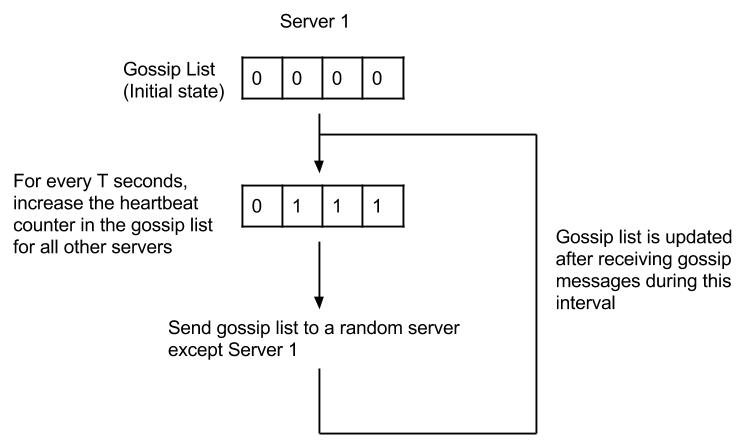
\includegraphics[scale=0.6]{gossip_send.jpg}
%\centering
%\caption{Gossip Module - Sending Gossip Message}
%\label{fig:sending_gmsg}
%\centering
%\end{figure}

\item Another server receiving gossip message will merge its local gossip list and the gossip list contained in gossip protocol message by adopting the minimum heartbeat counter for each known server as shown in Figure~\ref{fig:send_receive_gmsg}.

%\begin{figure}[h]
%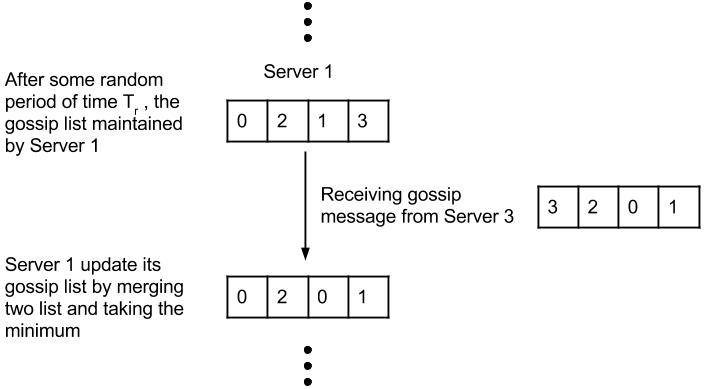
\includegraphics[scale=0.6]{gossip_receive.jpg}
%\centering
%\caption{Gossip Module - Receiving Gossip Message and Updating Gossip List}
%\label{fig:receiving_gmsg}
%\centering
%\end{figure}

\item At any point of time, if the difference between local heartbeat counter and the heartbeat counter of a remote server is greater than the error factor F, that particular remote server is suspected by the local server. For example, if the gossip list of \verb|server1| is \verb|{"1":0,"2":5,"3":1,"4":2}| when error factor F = 5, \verb|server1| suspects \verb|server2| has crashed. And SuspectList in \verb|server1| is updated as:
\begin{small}
\begin{verbatim}
SuspectList = {"1":NOT_SUSPECTED, "2":SUSPECTED, "3":NOT_SUSPECTED, "4":NOT_SUSPECTED}
\end{verbatim}
\end{small}

%\verb|SuspectList = {"1":NOT_SUSPECTED, "2":SUSPECTED, "3":NOT_SUSPECTED, "4":NOT_SUSPECTED}|

\end{enumerate}

\subsection{Comparison and Improvement}

This gossip based algorithm differs from the Naive failure detector such that instead of asking all other peers "Are you alive?", each server now only select a random peer to gossip and share its view of the global state to that server. Eventually, all the correct servers will have agreements on the global state of Strike system. For example, if \verb|server2| is crashed, the heartbeat counter of \verb|server2| maintained by the failure detector module of all the other servers will be higher count as no server receives messages from \verb|server2| and only \verb|server2| can reset its own heartbeat counter. Gossip-type protocol solves the problem of message explosion as the number of TCP connections/messages among servers during gossip interval T is only N for N servers, and complexity is reduced from $O({N^2})$ to $O(N)$, comparing to the Naive approach failure detector.

However, this algorithms scales in detection time. For N servers, the detection time increases $O(NlogN)$\cite{gossip} if T and F remains the same. Whereas for the Naive approach failure detector, the detection time is static no matter how $N$ grows. Another drawback is that when a large proportion of servers are crashed simultaneously, the failure detector will take much time to detect the failed servers by gossiping messages around.

It is also worth mentioning that we can modify the data structure of gossip list to store not only heartbeat counters but also \textbf{ServerInfo}\footnote{ServerInfo is a Java class in Strike storing server informations}. So as the servers are gossiping each other, they will gain more detail information about the global state of Strike servers. Nevertheless, there will be incremental in the size of gossip message. In terms of message size, it also downgrades the scalability of gossip protocol because when number of server increases, the size of serialized message buffer will increase.

Overall, gossip protocol sacrifice a lot to achieve reduction in messages comparing to Naive approach. There are other protocols such as Hierarchical approach and Lazy Failure Detection protocol\cite{failuredetector}. However, failure detector implemented with different protocols and algorithms is aimed to address different problems in different scenarios i.e. message explosion, scalability, message loss, etc. There is no perfect solution that solves all problems.

\end{document}